\documentclass{article}
\usepackage[margin=1in]{geometry}
\usepackage{fancyvrb}
\usepackage{multicol}
\usepackage{hyperref}
\usepackage{amsmath}
\usepackage{amsfonts}

\usepackage[listings]{tcolorbox}

\definecolor{codegreen}{rgb}{0,0.6,0}
\definecolor{codegray}{rgb}{0.5,0.5,0.5}
\definecolor{codepurple}{rgb}{0.58,0,0.82}
\definecolor{backcolour}{rgb}{0.95,0.95,0.92}

\lstdefinestyle{mystyle}{
    language=Python,
    backgroundcolor=\color{backcolour},   
    commentstyle=\color{codegreen},
    keywordstyle=\color{magenta},
    numberstyle=\tiny\color{codegray},
    stringstyle=\color{codepurple},
    basicstyle=\ttfamily\footnotesize,
    breakatwhitespace=false,         
    breaklines=true,                 
    captionpos=b,                    
    keepspaces=true,                 
    numbers=left,                    
    numbersep=5pt,                  
    showspaces=false,                
    showstringspaces=false,
    showtabs=false,                  
    tabsize=2,
    escapechar=|,
    frame=single
}

\lstset{style=mystyle}

\newcommand{\showfig}[2]{
\noindent\includegraphics[width=\textwidth]{#1}
\centerline{#1}
}
\newcommand{\bi}{\begin{itemize}}
\newcommand{\li}{\item}
\newcommand{\ei}{\end{itemize}}

\usepackage{graphicx}
\usepackage{hyperref,fancyvrb,amsmath}
\usepackage{tikz}
\usepackage{tikz-qtree}

\newcommand{\mydot}[1]{\draw[fill] (#1) circle (0.1);}

\newcommand{\set}[1]{\ensuremath{\{#1\}}}

\title{Faster Maze Solver}
\author{CSCI112, Lab 11}

\begin{document}

\maketitle
\centerline{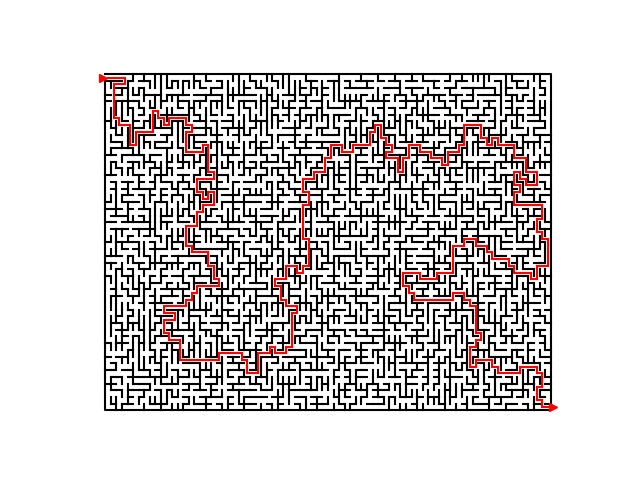
\includegraphics[scale=1]{Figure_1}}

\begin{description}

\item[File names:]  Names of files, functions, and variables, 
when specified,
must be EXACTLY as specified.  This includes simple mistakes such
as capitalization.

\item[Individual work:]  All work must be your own.  Do not share
code with anyone other than the instructor and teaching assistants.
This includes looking over shoulders at screens with the code open.
You may discuss ideas, algorithms, approaches, {\em etc.} with
other students but NEVER actual code.  Do not use code
written by anyone else, in the class or from the internet.

\item[Documentation:] Each file should begin with a docstring
that includes your name, the class number and name, the lab
number, and  
a short description of the lab, as well as documentation pertinent
to that particular file.

\item[Speeding up search with heuristics:]  When your depth-first
solver from last week was deciding which node to explore next,
it had no guidance at all from the maze itself.  A human will look
at the maze and use spatial reasoning to make reasonable
choices.  Not infallible choices, just reasonable ones.

We are going to give our maze solver a bit of intelligence by using
a priority queue for the gray cells instead of a stack.  Each node's
priority will be determined by the Manhattan distance from the goal.
Manhattan distance between two points is defined as follows:
\[
\mbox{manhattan}((x_1, y_1), (x_2, y_2)) =|x_1-x_2| + |y_1-y_2|
\]
where $|x|$ is the absolute value of $x$.

Our heuristic is that nodes that are {\em closer} to the goal are
more likely to be on the solution path than nodes that are {\em farther}.
We will accordingly use a min queue for the cells on the gray
list, and use the cell closest to the goal each time.

Technically this algorithm is called ``greedy,'' in that it tries
to make the biggest improvement possible with each step.
It takes nothing into account except getting closer to its goal!

\item[Timing:]  Run some experiments to see how much you've
speeded up the search.  In lieu of actual timing, you can 
compare the number of nodes added to the gray list before
termination.  The heuristic should reduce this.

\end{description}
\end{document}
